\documentclass[xcolor=dvipsnames]{beamer}
%\documentclass[handout,xcolor=dvipsnames,pdftex,hyperref={colorlinks=false}]{beamer}
\setbeamertemplate{items}[ball]
\setbeamertemplate{blocks}[rounded][shadow=true]
\usepackage{xcolor}
\usepackage{colortbl}
\usepackage{multirow}
\usepackage{amsmath,amsthm,amssymb}
\usepackage{amsfonts}
\usepackage{times}
\usepackage[T1]{fontenc}
\usepackage{bbm}
\usepackage[normalem]{ulem}
\usepackage{url}

\newcommand{\ra}{\rightarrow}
\newcommand{\la}{\leftarrow}
\newcommand{\lra}{\leftrightarrow}

\usepackage{tikz}
\usetikzlibrary{positioning}
\usetikzlibrary{shapes,decorations,arrows,calc,arrows.meta}
\tikzset{
  -latex,auto,node distance = 1.5cm and 1.5cm,
  semithick,
  state/.style ={ellipse, draw, minimum width = 0.5 cm},
  el/.style = {inner sep=2pt, align=left, sloped},
  point/.style = {circle, draw=black, inner sep=0.04cm,
   fill=black, node contents={}},
}

% == theme & colors
\usetheme{Warsaw}
\definecolor{someblue}{rgb}{0,.1,0.8}
\definecolor{dgreen}{rgb}{0,.6,0.8}

\newtheorem{arule}{Rule}
\newtheorem{iass}{Identification Assumption}

\newcommand\E{\mathbb{E}}
\newcommand{\indep}{{\bot\negthickspace\negthickspace\bot}}

\useoutertheme{infolines}

\title[DAGs]{Causal DAGs: the structural meaning of CI}
\subtitle[ ]{PS 200C, Spring 2026}
\author{Chad Hazlett}
\institute[UCLA]{UCLA\\[1ex]
  \texttt{chazlett@ucla.edu}}
\date{}

\begin{document}

\begin{frame}
  \titlepage
\end{frame}


%% =====================================================================
\section{Where we are}
%% =====================================================================

\begin{frame}{Where we are, and today's question}
\small
\onslide<1-> So far: \textbf{selection on observables}.  We assumed CI:
$$\{Y_{1i}, Y_{0i}\} \indep D_i \mid X_i$$
Then if we condition on the right $X$, treatment is as-if random within strata.\\[6pt]

\onslide<2-> Today we talk about graphical causal models (``DAGs'') that help show:
\begin{itemize}
\footnotesize
\item<2-> \textbf{Which} $X$ is the ``right'' $X$?
\item<3-> Is any $X$ good enough?
\item<3-> What can \textbf{go wrong} if I pick certain $X$?
\end{itemize}

\bigskip
\onslide<4-> \textcolor{Blue}{Core idea:} Ask \textit{why} $D$ and $Y$ could be associated. Three possibilities:
\begin{enumerate}
\footnotesize
\item<4-> $D$ causes $Y$ --- the effect we want.
\item<5-> A \textbf{common cause} of $D$ and $Y$.
\item<6-> Analytic errors that create these associations. 
\end{enumerate}

\onslide<7-> DAGs visualize and tell us how to remove unwanted sources of association. 
\end{frame}


%% =====================================================================
\section{Motivation: confounding, seen two ways}
%% =====================================================================

\begin{frame}{Confounding, with numbers}
\small
\onslide<1-> Suppose people self-select into a new drug.  You find:
\begin{table}
\footnotesize
\centering
\begin{tabular}{l|c|c|}
\cline{2-3}
 & \multicolumn{2}{c|}{\textit{Recovered} (count / total)} \\ \cline{2-3}
 & Drug & No drug \\ \hline
\multicolumn{1}{|l|}{Mild}     & 81 of 87 (93\%)  & 234 of 270 (87\%) \\ \hline
\multicolumn{1}{|l|}{Severe}   & 192 of 263 (73\%) & 55 of 80 (69\%) \\ \hline
\multicolumn{1}{|l|}{Combined} & 273 of 350 (78\%) & 289 of 350 (83\%) \\ \hline
\end{tabular}
\end{table}

\onslide<2-> Pooled, the drug ``hurts'' (78 vs 83), but within each severity stratum the drug helps (93 vs 87; 73 vs 69).\\
\bigskip
\onslide<4-> \textcolor{Blue}{Why?} The pooled comparison compares groups that differ in \textit{severity}, not just the drug.\\
\bigskip
\onslide<5-> With POMs, we might have noted that $\E[Y(0)|D=1]-\E[Y(0)|D=0] < 0$ (negative bias)\\
\end{frame}


\begin{frame}{Preview: Confounding, with a DAG}

\
\medskip
\onslide<1-> What we \textit{believe} about the world:
\begin{itemize}
\footnotesize
\item Severity increases drug-taking
\item Severity causes reduced recovery
\item The drug might cause recovery.
\end{itemize}

\onslide<2->
\begin{center}
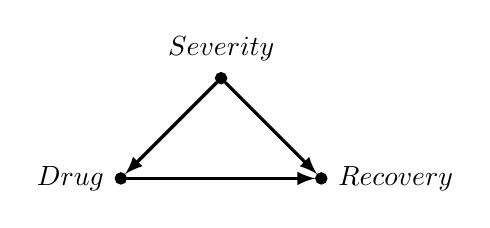
\begin{tikzpicture}[node distance = 1.8cm, very thick]
  \node (S)  [label = above:$Severity$, point];
  \node (D) [label = left:$Drug$, below left of = S, point];
  \node (Y) [label = right:$Recovery$, below right of = S, point];
  \path (S) edge (D);
  \path (S) edge (Y);
  \path (D) edge (Y);
\end{tikzpicture}
\end{center}

\onslide<3-> Now you can \textit{see} the two reasons $Drug$ and $Recovery$ are associated:
\begin{enumerate}
\footnotesize
\item $Drug \to Recovery$ (what we want),
\item $Drug \la Severity \to Recovery$ (common cause --- a spurious association).
\end{enumerate}

\onslide<4-> Conditioning on $Severity$ removes (2), leaving only (1).
\end{frame}


%% =====================================================================
\section{What's a DAG}
%% =====================================================================

\begin{frame}{What's a DAG?}
\small
A \textbf{Directed Acyclic Graph} (DAG):
\begin{itemize}
\footnotesize
\item<1-> \textbf{Nodes} = variables.
\item<2-> \textbf{Arrows, Edges} = direct causal relationships ($A \to B$: $A$ is a direct cause of $B$).
\item<3-> \textbf{No cycles}: you can't follow arrows and end up back where you started.
\item<4-> \textbf{Missing arrows encode assumptions}: ``$A$ is \textit{not} a direct cause of $B$.''  These are the assumptions doing the real work.
\item<5-> \textbf{Dashed arrow / bidirected arc} = unobserved common cause.
\end{itemize}

\bigskip
\onslide<6-> Three things a DAG is \textit{not}:
\begin{itemize}
\footnotesize
\item Not a list of the variables in your dataset.  (Many nodes may be unobserved.)
\item Not a statistical model.  (No parametric assumptions.)
\item Not a complete theory of the world.  (Just enough structure for the causal claim you want to make.)
\end{itemize}
\end{frame}


%% =====================================================================
\section{Three ways $D$ and $Y$ can be associated}
%% =====================================================================

\begin{frame}{Three path types}
\small
A ``path'' between two nodes is any sequence with edges connecting them (in any direction). Three elementary components of paths:

\bigskip
\onslide<2->
\begin{itemize}
\item \textcolor{Blue}{\textbf{Chain}}: $A \to B \to C$
\medskip
\item \textcolor{Blue}{\textbf{Fork}} (common cause): $A \la B \to C$
\medskip
\item \textcolor{Blue}{\textbf{Collider}} (common effect): $A \to B \la C$
\end{itemize}

\bigskip
\onslide<3-> Our task: figure out, for each, (a) when is $A$ associated with $C$?  (b) what happens when we condition on $B$?
\end{frame}


\begin{frame}{Chain}
\small
$A \to B \to C$:
\begin{center}
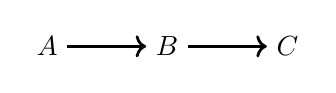
\begin{tikzpicture}
\node[text centered] (A) {$A$};
\node[right = 1 of A] (B) {$B$};
\node[right = 1 of B] (C) {$C$};
\draw[->, line width= 1] (A) -- (B);
\draw[->, line width= 1] (B) -- (C);
\end{tikzpicture}
\end{center}

\medskip
\onslide<2-> $A \indep C$? \onslide<3-> \textcolor{Red}{No} --- $A$ affects $C$ through $B$.\\
\medskip
\onslide<4-> $A \indep C \mid B$? \onslide<5-> \textcolor{Green}{Yes} --- conditioning on $B$ blocks the chain.\\
\medskip
\onslide<6-> \textit{Moral}: a chain transmits association; conditioning on the middle blocks it.
\end{frame}


\begin{frame}{Fork (common cause)}
\small
$A \la B \to C$:
\begin{center}
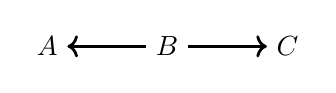
\begin{tikzpicture}
\node[text centered] (A) {$A$};
\node[right = 1 of A] (B) {$B$};
\node[right = 1 of B] (C) {$C$};
\draw[->, line width= 1] (B) -- (A);
\draw[->, line width= 1] (B) -- (C);
\end{tikzpicture}
\end{center}

\medskip
\onslide<2-> $A \indep C$? \onslide<3-> \textcolor{Red}{No} --- the common cause $B$ induces association.\\
\medskip
\onslide<4-> $A \indep C \mid B$? \onslide<5-> \textcolor{Green}{Yes} --- conditioning on the common cause blocks it.\\
\medskip
\onslide<6-> \textit{Moral}: a common cause creates spurious association; conditioning on it removes it.  \textbf{This is classical confounding.}
\end{frame}


\begin{frame}{Collider (common effect)}
\small
$A \to B \la C$:
\begin{center}
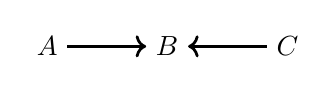
\begin{tikzpicture}
\node[text centered] (A) {$A$};
\node[right = 1 of A] (B) {$B$};
\node[right = 1 of B] (C) {$C$};
\draw[->, line width= 1] (A) -- (B);
\draw[->, line width= 1] (C) -- (B);
\end{tikzpicture}
\end{center}

\medskip
\onslide<2-> $A \indep C$? \onslide<3-> \textcolor{Green}{Yes} --- no causal path, no common cause.\\
\medskip
\onslide<4-> $A \indep C \mid B$? \onslide<5-> \textcolor{Red}{\textbf{No!}} --- conditioning on the collider \textit{opens} a path.\\

\bigskip
\onslide<6-> \textit{Moral}: colliders are the reverse of the other two.  They are \textit{already blocked}, and conditioning on one \textit{creates} an association that wasn't there.
\end{frame}


\begin{frame}{Colliders are real}
\footnotesize
\onslide<1-> \textbf{Pearl's favorite}:
\begin{itemize}
\item[] Rain $\to$ Wet lawn $\la$ Sprinkler was on
\end{itemize}
Observing a wet lawn, learning it did \textit{not} rain raises the chance the sprinkler ran.

\bigskip

\onslide<2-> \textbf{Hollywood}:
\begin{itemize}
\item[] Looks $\to$ Fame $\la$ Talent
\end{itemize}
Among famous actors, the good-looking ones are less talented (on average).

\bigskip

\onslide<3-> \textbf{Academic tenure}:
\begin{itemize}
\item[] Productivity $\to$ Tenure $\la$ Originality
\end{itemize}
Among tenured faculty, the prolific ones are less original (on average).

\bigskip

\onslide<4-> \textcolor{Blue}{Lesson}: Conditioning on something can give rise to a spurious association...this will matter when we start trying to isolate causal effects.
\end{frame}


\begin{frame}{A collider in the wild}
\begin{figure}[h!]
\begin{center}
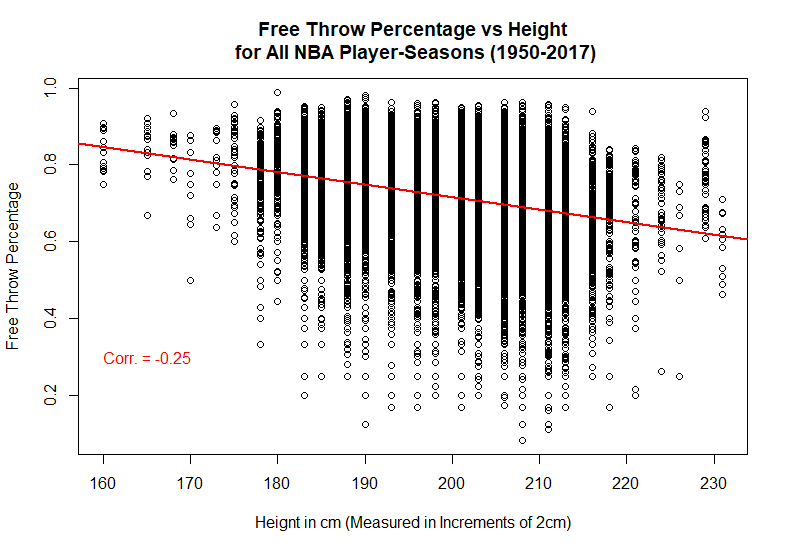
\includegraphics[scale=0.42]{figures/Free Throw Percentage vs Height.png}
\end{center}
\end{figure}

\onslide<2-> Why do you think that is?  Answer with a DAG.\\
\medskip
\footnotesize
\textit{Source: Adam Rohde, via \texttt{basketball-reference.com} and kaggle.com/datasets/drgilermo/nba-players-stats.}
\end{frame}


%% =====================================================================
\section{d-separation: when does conditioning kill all the paths?}
%% =====================================================================

\begin{frame}{$d$-separation}
\small
Putting the three patterns together:
\begin{arule}
\textbf{$d$-separation.}  $A$ and $C$ are $d$-separated by a set $Z$ iff \textit{every path} between them is blocked.  A path is blocked when:
\begin{itemize}
\footnotesize
\item It contains a \textit{chain} or \textit{fork} at a node in $Z$, \textbf{or}
\item It contains a \textit{collider} such that neither the collider nor any descendant of it is in $Z$.
\end{itemize}
\end{arule}

\bigskip
\onslide<2-> If $A$ and $C$ are $d$-separated by $Z$, then
$$A \indep C \mid Z$$

\medskip
\onslide<3-> \textit{In plain English}: When $A$ and $C$ are d-separated by $Z$ in this way, you can condition on $Z$ as a way to remove the association between $A$ and $C$ due to those paths.
\end{frame}


\begin{frame}{Practice: $d$-separation}
\begin{center}
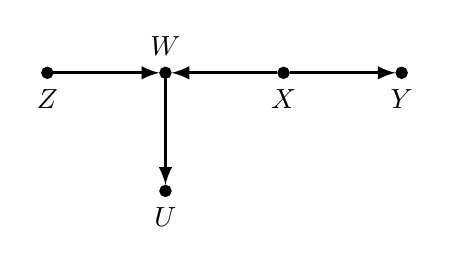
\begin{tikzpicture}[very thick]
\node (z)  [label = below:$Z$, point];
\node (w) [label = above:$W$, right of = z, point];
\node (x) [label = below:$X$, right of = w, point];
\node (y) [label = below:$Y$, right of = x, point];
\node (u) [label = below:$U$, below of = w, point];
\path (z) edge (w);
\path (x) edge (w);
\path (w) edge (u);
\path (x) edge (y);
\end{tikzpicture}
\end{center}

\small
Looking at $Z$ and $Y$:
\begin{itemize}
\item<2-> $d$-separated by $\{\}$? \onslide<3-> \textcolor{Green}{Yes} --- the only path is $Z\!\to\!W\!\la\!X\!\to\!Y$, with $W$ as collider; no conditioning $\Rightarrow$ blocked.
\item<4-> $d$-separated by $\{W\}$? \onslide<5-> \textcolor{Red}{No} --- conditioning on the collider $W$ \textit{opens} the path.
\item<6-> $d$-separated by $\{W, X\}$? \onslide<7-> \textcolor{Green}{Yes} --- $W$ opens $Z\text{-}Y$, but $X$ (a chain node on that path) re-blocks it.
\item<8-> $d$-separated by $\{U\}$? \onslide<9-> \textcolor{Red}{No} --- $U$ is a descendant of collider $W$, so conditioning on it also opens the path.
\end{itemize}
\end{frame}


\begin{frame}{Back to the big picture}
\small
\onslide<1-> You do some analysis and see that $D$ and $Y$ associated. But is this down to $D \rightarrow Y$, or something else? 

\bigskip
\onslide<2-> \textbf{What we want}: a rule for choosing  set $\{X\}$ such that, after conditioning, the \textit{only} remaining association between $D$ and $Y$ is the causal arrow $D \to Y$.

\bigskip
\onslide<3-> That rule is the \textbf{backdoor criterion}.
\end{frame}


%% =====================================================================
\section{Backdoor = CI}
%% =====================================================================

\begin{frame}{Front-door and back-door paths}
\small
\begin{itemize}
\item<1-> A \textcolor{Blue}{\textbf{frontdoor path}} from $D$ to $Y$ starts with an arrow \textit{out of} $D$.  These carry causation.  We want to \textbf{leave them open}.
\medskip
\item<2-> A \textcolor{Blue}{\textbf{backdoor path}} from $D$ to $Y$ starts with an arrow \textit{into} $D$.  These carry spurious association.  We want to \textbf{block them all}.
\end{itemize}

\bigskip
\onslide<3->
\begin{center}
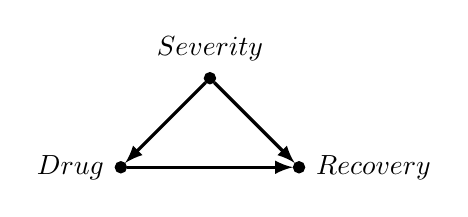
\begin{tikzpicture}[node distance = 1.6cm, very thick]
  \node (S)  [label = above:$Severity$, point];
  \node (D) [label = left:$Drug$, below left of = S, point];
  \node (Y) [label = right:$Recovery$, below right of = S, point];
  \path (S) edge (D);
  \path (S) edge (Y);
  \path (D) edge (Y);
\end{tikzpicture}
\end{center}

\footnotesize
\onslide<4-> Frontdoor: $Drug \to Recovery$.\\
\onslide<5-> Backdoor: $Drug \la Severity \to Recovery$.  Condition on $Severity$ to block it.
\end{frame}


\begin{frame}{The backdoor criterion}
\small
\onslide<1->
\begin{arule}
\textbf{Backdoor criterion.} $\{X\}$ satisfies the backdoor criterion relative to $(D, Y)$ if:
\begin{enumerate}
\footnotesize
\item No node in $X$ is a descendant of $D$ \textcolor{gray}{(don't block frontdoor paths)}, \textbf{and}
\item $X$ blocks every backdoor path from $D$ to $Y$.
\end{enumerate}
\end{arule}

\bigskip
\onslide<2-> For humans, find a set $X$ that:
\begin{enumerate}
\footnotesize
\item<2-> blocks all \textit{spurious} paths (every backdoor),
\item<3-> leaves \textit{causal} paths untouched (no descendants of $D$),
\item<4-> doesn't \textit{open new} spurious paths (no colliders or their descendants unless paired with another blocker downstream).
\end{enumerate}
\end{frame}


\begin{frame}{Backdoor = CI: two languages, one object}
\small
\onslide<1-> \textbf{Theorem (informal)}\footnote{For formal statements: Pearl, Glymour \& Jewell (2016) \textit{Primer} Thm 4.3.1; Shpitser, VanderWeele \& Robins (2010) adjustment criterion.}: if $X$ satisfies the backdoor criterion in a DAG, then
$$\{Y_{1i}, Y_{0i}\} \indep D_i \mid X_i$$
in any SCM consistent with that DAG.\\[4pt]

\onslide<2-> We can then apply the ``adjustment formula'' if we wanted to recover $P(Y)$ as if we ``made everyone have treatment $D=d$'', i.e. $P(Y \mid do(d))$:
$$P(Y \mid do(d)) = \sum_x P(Y \mid D\!=\!d, X\!=\!x)\,P(X\!=\!x).$$
Or, since we have been working with expectations:
$$\E(Y \mid do(d)) = \sum_x \E(Y \mid D\!=\!d, X\!=\!x)\,P(X\!=\!x)$$
\end{frame}

\begin{frame}{Adjustment formula for ATE}
\onslide<1-> If you use this to get the ATE, $\E[Y \mid do(D=1)]-\E[Y \mid do(D=0)]$, you see exactly what we say with adjustment under SOO:\\

$$ \sum_x \left(\E[Y \mid D\!=\!1, X\!=\!x]-\E[Y \mid D\!=\!0, X\!=\!x]\right)\,P(X\!=\!x)$$


\medskip
\onslide<2-> That is: figuring out what to condition on using the DAG and adjusting for it is the same thing we were doing by (i) claiming CI given those variables and (ii) conditioning on them.\\

\bigskip

\onslide<3-> As before, sub-stratification is the literal way to do so, but in practice we'll often need to use other approaches that give us an estimate as if $p(X|D=1)$ and $p(X|D=0)$.\\



\end{frame}

%% =====================================================================
\section{Four examples}
%% =====================================================================

\begin{frame}{Example 1: a hidden confounder, but a workable adjustment set}
\onslide<1->
\begin{center}
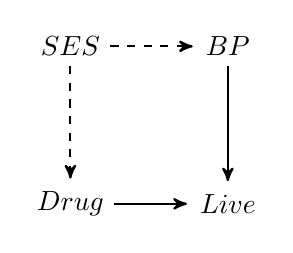
\begin{tikzpicture}[-,>=stealth',shorten >=1pt,auto,node distance=2cm,
  thick,main node/.style={circle,fill=blue!20,draw,font=\sffamily\Large\bfseries}]
  \node (x) {$Drug$};
  \node (z) [above of=x] {$SES$};
  \node (w) [right of=z] {$BP$};
  \node (y) [right of=x] {$Live$};
  \draw[->] (x) -- (y);
  \draw[->] (w) -- (y);
  \draw[dashed, ->] (z) -- (x);
  \draw[dashed, ->] (z) -- (w);
\end{tikzpicture}
\end{center}
\footnotesize
$SES$ unobserved (dashed).  Can we identify the effect of $Drug$ on $Live$?

\small
\begin{itemize}
\item<2-> Backdoor paths? \onslide<3-> $Drug \la SES \to BP \to Live$
\item<4-> Observed set that blocks it? \onslide<5-> $\{BP\}$
\item<6-> Equivalent CI statement: $\{Live_{1}, Live_{0}\} \indep Drug \mid BP$.
\end{itemize}
\end{frame}


\begin{frame}{Example 2: multiple valid adjustment sets}
\onslide<1->
\begin{center}
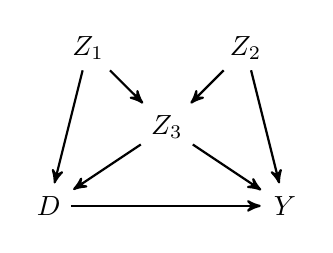
\begin{tikzpicture}[->,>=stealth',shorten >=1pt,auto,node distance=2cm,
  thick,main node/.style={circle,fill=blue!20,draw,font=\sffamily\Large\bfseries}]
\node at (0,0) (X) {$D$};
\node at (3,0) (Y) {$Y$};
\node at (.5,2) (Zone) {$Z_1$};
\node at (2.5,2) (Ztwo) {$Z_2$};
\node at (1.5,1) (Zthree) {$Z_3$};
\draw[->, line width=.8] (X) -- (Y);
\draw[->, line width=.8] (Zone) -- (X);
\draw[->, line width=.8] (Ztwo) -- (Y);
\draw[->, line width=.8] (Zone) -- (Zthree);
\draw[->, line width=.8] (Ztwo) -- (Zthree);
\draw[->, line width=.8] (Zthree) -- (X);
\draw[->, line width=.8] (Zthree) -- (Y);
\end{tikzpicture}
\end{center}
\small
\begin{itemize}
\item<2-> Backdoor paths? $D \la Z_1 \to Z_3 \to Y$; $D \la Z_3 \to Y$; $D \la Z_3 \la Z_2 \to Y$.
\item<3-> Several valid sets: $\{Z_3\}$, $\{Z_1, Z_2\}$, $\{Z_3, Z_1\}$, \ldots
\item<4-> \textit{Invariance}: all give you the same estimand in the non-parametric sense.  Different estimators in practice, though.
\end{itemize}
\end{frame}


\begin{frame}{Example 3: How about now?}
\onslide<1->
\begin{center}
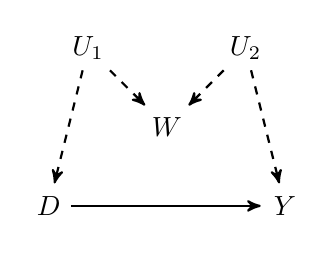
\begin{tikzpicture}[->,>=stealth',shorten >=1pt,auto,node distance=2cm,
  thick,main node/.style={circle,fill=blue!20,draw,font=\sffamily\Large\bfseries}]
\node at (0,0) (X) {$D$};
\node at (3,0) (Y) {$Y$};
\node at (0.5,2) (Uone) {$U_1$};
\node at (1.5,1) (W) {$W$};
\node at (2.5,2) (Utwo) {$U_2$};
\draw[->, line width=.8] (X) -- (Y);
\draw[dashed, ->] (Uone) -- (X);
\draw[dashed, ->] (Uone) -- (W);
\draw[dashed, ->] (Utwo) -- (W);
\draw[dashed, ->] (Utwo) -- (Y);
\end{tikzpicture}
\end{center}
\small
\begin{itemize}
\item<2-> Backdoor paths?  The only candidate is $D \la U_1 \to W \la U_2 \to Y$.
\item<3-> $W$ is a collider on that path, so the path is \textcolor{Blue}{already blocked}.  Empty set suffices!
\item<4-> What if your colleague says, ``let's play it safe and condition on $W$''? \onslide<5-> \textcolor{Red}{You open it.}  Now $D$ and $Y$ are spuriously associated through the (now unblocked) $U_1, U_2$.
\end{itemize}

\medskip
\onslide<6-> Lessons: 1. DAGs help you see if CI holds; and 2. Conditioning on extra variables can \textit{break} an identification that was fine without them.
\end{frame}


\begin{frame}{Example 4: Failure of identification}
\onslide<1->
\begin{center}
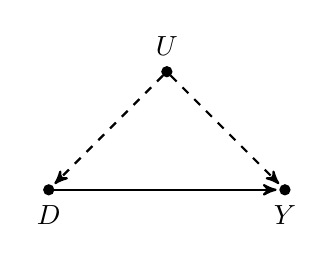
\begin{tikzpicture}[->,>=stealth',shorten >=1pt,auto,node distance=2cm,
  thick,main node/.style={circle,fill=blue!20,draw,font=\sffamily\Large\bfseries}]
\node at(1.5,1.5) (U) [label = above:$U$, point];
\node at(0,0) (X) [label = below:$D$, point];
\node at(3,0) (Y) [label = below:$Y$, point];
\draw[dashed, ->] (U) -- (X);
\draw[dashed, ->] (U) -- (Y);
\path (X) edge (Y);
\end{tikzpicture}
\end{center}
\small
\begin{itemize}
\item<2-> Backdoor path: $D \la U \to Y$.  $U$ unobserved.
\item<3-> No observed variable blocks it.  \textcolor{Red}{No set satisfies the backdoor criterion.}
\end{itemize}

\bigskip
\onslide<4-> DAGs tell you when you're stuck --- not just when you're fine. \\
\bigskip
\onslide<5->  What to do? SOO+sensitivity, or find another ID strategy.
\end{frame}


%% =====================================================================
\section{Complaints and responses}
%% =====================================================================

\begin{frame}{Complaints (and responses)}
\small
\onslide<1-> \textit{``I can't really know the true causal structure.''}\\
\smallskip
\onslide<2-> True.  But SOO isn't any different...you can't support it with claiming ausal structure. Drawing the DAG forces you to be \textit{explicit} about what you're assuming.  Different people can then disagree productively, not just pick different controls silently.

\bigskip
\onslide<3-> \textit{``I've always worked with potential outcomes, not DAGs.''}\\
\smallskip
\onslide<4-> They're two languages for the same object.  CI = backdoor; the adjustment formula = stratification.  DAGs are especially good at spotting \textit{traps} (colliders, post-treatment conditioning) that are hard to see in PO notation.

\bigskip
\onslide<5-> \textit{``Different people draw different DAGs.''}\\
\smallskip
\onslide<6-> This is a feature not a bug: the DAG is surfacing key disagreement that needs to be resolved or what-if'd out.
\end{frame}


%% =====================================================================
\section{Wrap}
%% =====================================================================

\begin{frame}{Resources: going deeper}
\small
\onslide<1-> Today was a quick practical tour.  For more practice or details:\\[4pt]

\onslide<2-> \textbf{Books}:
\begin{itemize}
\footnotesize
\item \textit{What If} (Hern\'an and Robins, 2024).  Chapters 6, 7.  Free online.
\item \textit{Causal Inference in Statistics: A Primer} (Pearl, Glymour, Jewell, 2016).  Chapters 1.4, 1.5, 2, 3.
\item \textit{Causality} (Pearl, 2009).  The full treatment.
\end{itemize}

\bigskip
\onslide<3-> \textbf{Online courses / lectures}:
\begin{itemize}
\footnotesize
\item \textit{Causal Diagrams: Draw Your Assumptions Before Your Conclusions} --- Miguel Hern\'an, EdX.
\item \textit{A Crash Course in Causality} --- Jason Roy, Coursera.
\item *Richard McElreath, ``Science Before Statistics: Causal Inference.''\\
\url{https://www.youtube.com/watch?v=KNPYUVmY3NM}
\item *Richard McElreath, \textit{Statistical Rethinking} lecture series on YouTube (more on DAGs + Bayesian modeling).
\end{itemize}
\end{frame}


\begin{frame}{Takeaways}
\small
\begin{itemize}
\item<1-> \textbf{``Why are $D$ and $Y$ associated?''}  A DAG enumerates the answers: causal, common cause, or something else (e.g. a collider trap).
\medskip
\item<2-> \textbf{Paths come in three flavors}: chains and forks transmit association; colliders block it (and conditioning flips them).
\medskip
\item<3-> \textbf{$d$-separation} is the bookkeeping: does your conditioning set kill every path you don't want?
\medskip
\item<4-> \textbf{Backdoor criterion = CI}.  Same statement, two languages.  The DAG gives CI its structural meaning.
\medskip
\item<5-> \textbf{Conditioning can backfire}.  Collider conditioning, post-treatment conditioning.  More $X$ is not always better.
\medskip
\item<6-> \textbf{The graph tells you when you're stuck}.  Example 4 is the honest payoff: identification isn't guaranteed.
\end{itemize}
\end{frame}


\end{document}
